\documentclass[11pt,a4]{report}
\usepackage[utf8]{inputenc}
\usepackage[T1]{fontenc}
\usepackage[norsk]{babel}
%\renewcommand{\rmdefault}{cmss}    %forandrer font til times roma
\usepackage{verbatim,amsmath}
\usepackage{enumerate}
\usepackage{fancyhdr,fancyvrb}
\usepackage{graphicx,color,boxedminipage}
\usepackage{ragged2e,colortbl,appendix}
\usepackage{here,hyperref,multirow,pdfpages}
\usepackage[font=small,labelfont=bf]{caption}

\usepackage{xcolor}
\usepackage{lipsum,todonotes} 

% viser til figurer ligger 
%\usepackage[../FigurerFraProsjektene/DiverseFigurer/, 
%../FigurerFraProsjektene/MineFunksjoner/,
%../FigurerFraProsjektene/Prosjekt01_NumeriskIntegrasjon/,
%../FigurerFraProsjektene/Prosjekt02_Filtrering/,
%]{figurepath} 

% Her utvider du med nye mapper


% inkludering av kode 
\usepackage{listings}
%\usepackage[framed,numbered,autolinebreaks,useliterate]{mcode}
% for å kunne skrive norske kommentarer i Matlab og vises i listingspakken
%\lstset{inputencoding=ansinew}

% Default fixed font does not support bold face
\DeclareFixedFont{\ttb}{T1}{txtt}{bx}{n}{12} % for bold
\DeclareFixedFont{\ttm}{T1}{txtt}{m}{n}{12}  % for normal

% Custom colors
\usepackage{color}
\definecolor{deepblue}{rgb}{0,0,0.5}
\definecolor{deepred}{rgb}{0.6,0,0}
\definecolor{deepgreen}{rgb}{0,0.5,0}

\renewcommand{\figurename}{Fig.}

% Python style for highlighting
\newcommand\pythonstyle{\lstset{
language=Python,
basicstyle=\ttm,
morekeywords={self},              % Add keywords here
keywordstyle=\ttb\color{deepblue},
emph={MyClass,__init__},          % Custom highlighting
emphstyle=\ttb\color{deepred},    % Custom highlighting style
stringstyle=\color{deepgreen},
frame=tb,                         % Any extra options here
showstringspaces=false
}}

% Python environment
\lstnewenvironment{python}[1][]
{
\pythonstyle
\lstset{#1}
}
{}


\definecolor{darkgreen}{rgb}{0.0, 0.6, 0.0}
\definecolor{darkred}{rgb}{0.6, 0.0, 0.0}
\definecolor{gray}{rgb}{0.6, 0.6, 0.6}
\definecolor{mygreen}{RGB}{28,172,0} % color values Red, Green, Blue
\definecolor{mylilas}{RGB}{170,55,241}


% kan definere bredere tekstbredde og -høyde 
\textwidth135mm
\textheight195mm
\parindent0mm  % ingen innrykk ved begynnelsen av avsnitt

\setlength{\marginparwidth}{3cm}

\DeclareUnicodeCharacter{2212}{-}

\begin{document}
\setlength{\parskip}{0.5cm}   % denne lager 5mm avstand ved avsnitt
\selectlanguage{english}

% topptekst
\pagestyle{fancyplain}
\renewcommand{\chaptermark}[1]{\markboth{#1}{#1}}
\renewcommand{\sectionmark}[1]{\markright{\thesection\ #1}}
\lhead[\fancyplain{}{\bfseries\thepage}]{\fancyplain{}{\bfseries\rightmark}}
\rhead{}
\chead{}
\cfoot{\bfseries\thepage}
\lfoot{}
\rfoot{}


\renewcommand{\lstlistingname}{Kode}% Listing -> Kode


% forsidetabell
\begin{table}[hb]
	\centering
              \begin{tabular}{|l|lll|}\hline
                \multicolumn{4}{|l|}{\hspace*{130mm}}\\
                \multicolumn{4}{|l|}{DAT250}\\[-7mm]
                \multicolumn{4}{|r|}{\scalebox{0.4}}\\[15mm]
                \multicolumn{4}{|c|}{\Huge \bf PROSJEKT - HØSTEN 2021}\\[5mm]\hline
                & & &  \\[-3mm]
                Prosjekt- & \multicolumn{3}{|l|}{Project 1, Website security} \\
                oppgaven & \multicolumn{3}{|l|}{}\\[2mm]\hline
                \multicolumn{4}{c}{}\\[5mm]\hline
                & & &  \\[-3mm]
                Gruppenavn & \multicolumn{3}{|l|}{\color{red}{Gruppe 15, AlphaBank}} \\[2mm]\hline
                & & &\\[-3mm]
                Gruppens  & Navn &  Studentnummer & \\
                medlemmer  &   &   &  \\[2mm]
                & Matias Ramsland & 259150     &  \\[6mm]
                & Lukasz Pietkiewicz & 253469     &  \\[6mm]
                & Chiran Pokhrel & 259205     &  \\[6mm]
                & Jakub Mroz  & 260703       & \\[6mm]
                & Konrad Jarczyk & 242615 & \\[20mm]
                 \hline
              \end{tabular}
\end{table}


% ingen sidetall på forsiden
\thispagestyle{empty}

\newpage

% romerske tall før kap.1
\pagenumbering{roman} 
  
% Innholdsfortegnelse
% Første linje legger selve innholdsfortegnelsen inn i
% innholdsfortegnelsen. Dette må gjøres manuelt på de kapitlene
% uten nummer

\addcontentsline{toc}{chapter}{\protect\numberline{}Innhold} 
\tableofcontents

\newpage


\chapter*{Introduction}\label{kap:introduction}


The goal of the project was to create a secure banking application, resistant to OWASP TOP10 attacks.

Our application allows users to add money to their account,  send it to a different user through a webpage. Visitors cannot use banking services. To become a user, a visitor must sign up for an account first.

The application is written in python with flask framework, and is using SQLAlchemy with Heroku addon resource Heroku-Postgresql as our database where we store our information. 

% Siden sammendraget er uten kapittelnummer, legges dette manuelt inn
% i innholdsfortegnelsen
\addcontentsline{toc}{chapter}{\protect\numberline{}Introduction}

\newpage


% start vanlig nummering
% Side 1 skal ALLTID være der hvor kapittel 1 starter
\pagenumbering{arabic}

% rett høyre- og venstremarg
\justifying

% ingen innrykk ved nytt avsnitt
\setlength{\parindent}{0em} 

\chapter{Threat model and site map}\label{kap:Threat model and site map}

\renewcommand{\figurename}{Fig.}


\begin{figure}[H]
    \centering
    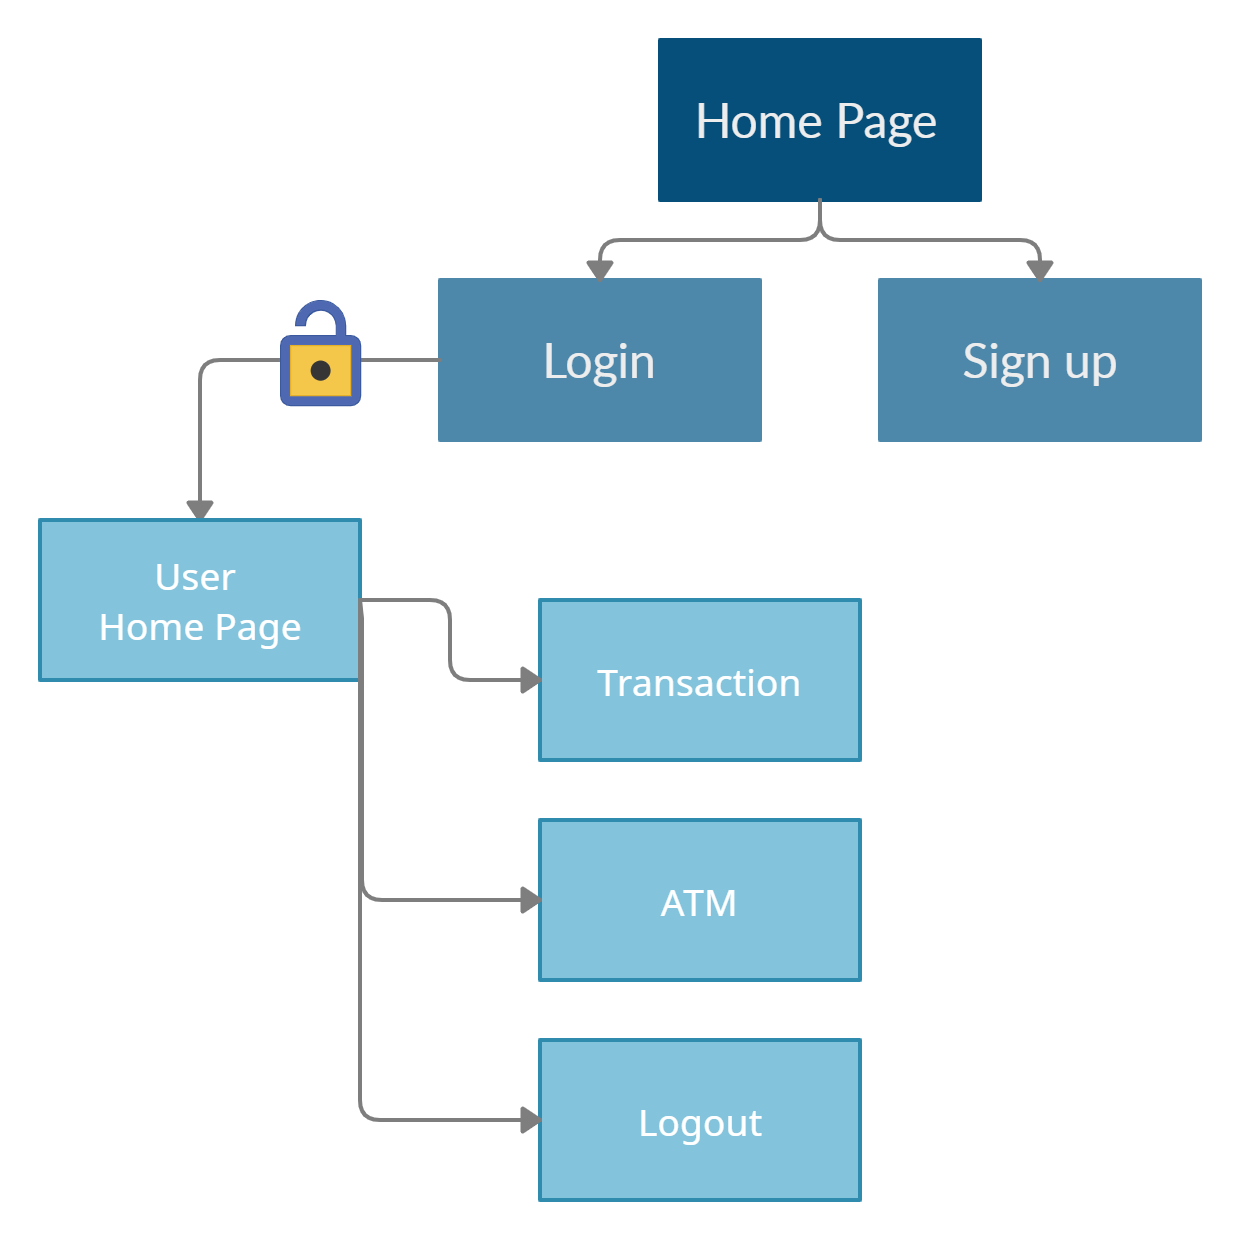
\includegraphics[width=\textwidth]{pics/pic1 Site map.png}
    \caption{Site map}
    \label{fig:kap1fig1sitemap}
\end{figure}

A visitor can only see login and signup pages from the homepage. When an unlogged user tries to visit the URL of any other page, he gets redirected back to the homepage.

\begin{figure}[H]
    \centering
    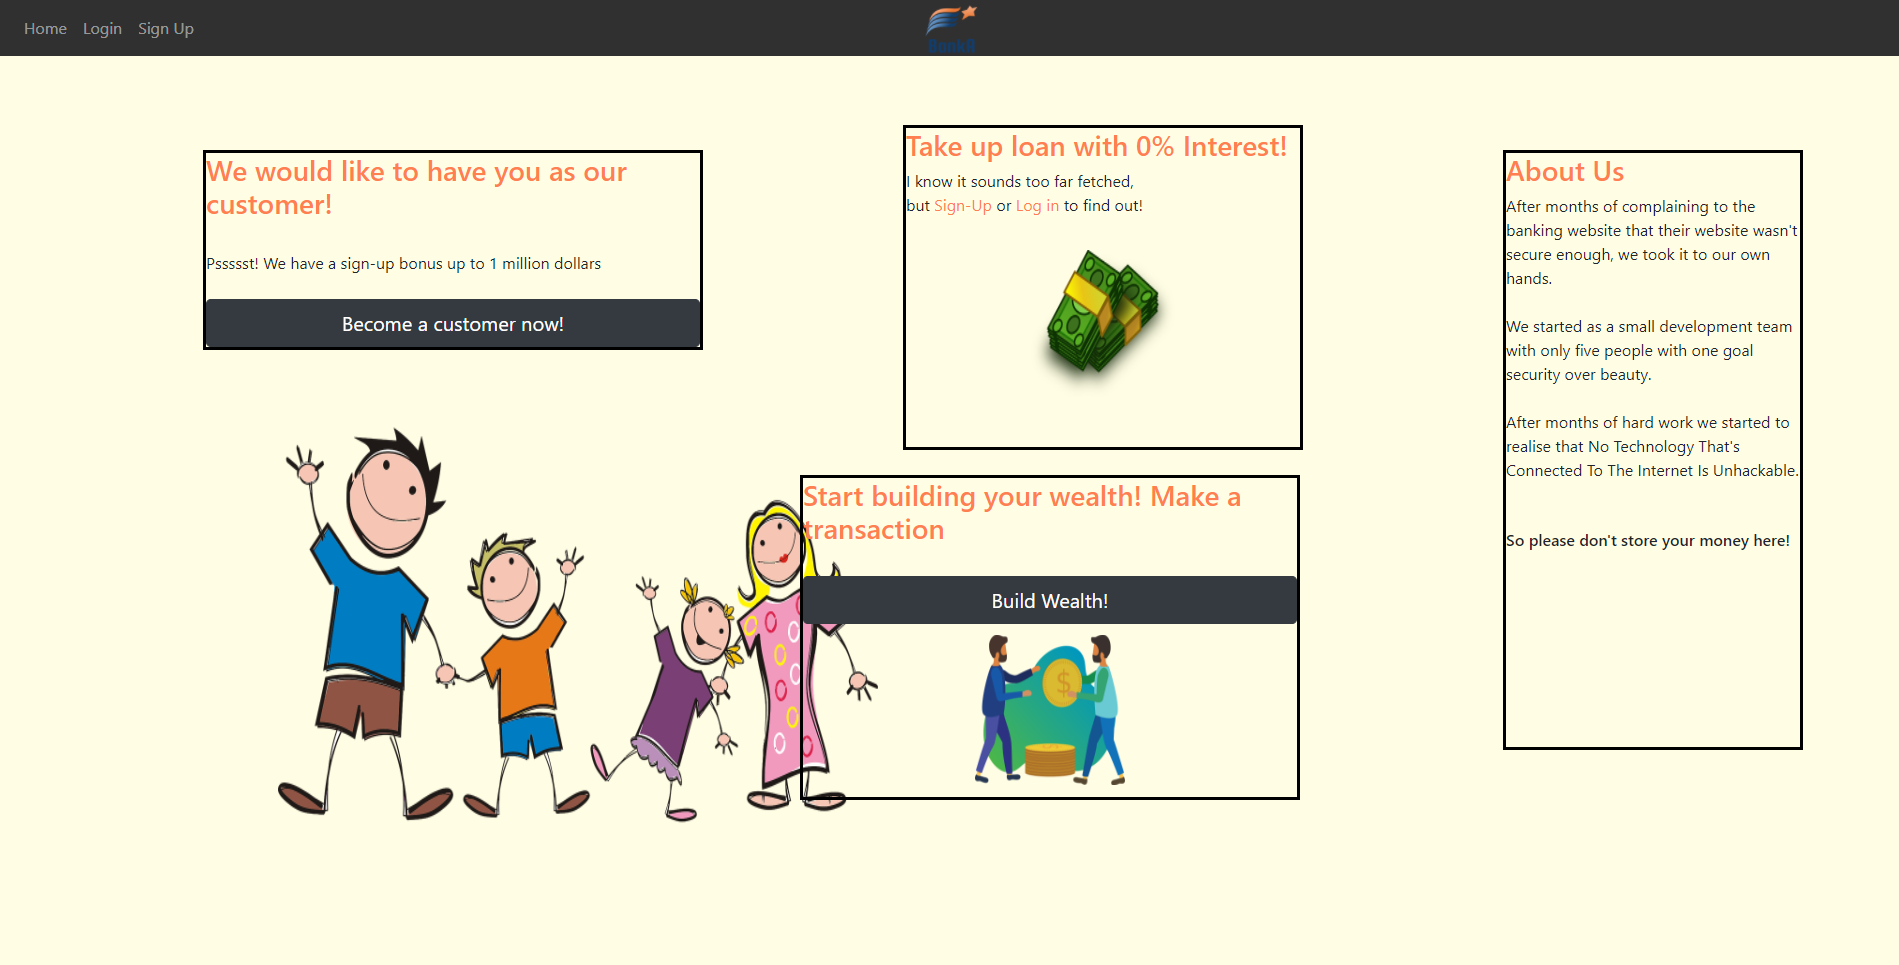
\includegraphics[width=\textwidth]{pics/pic2 home visitor.PNG}
    \caption{Site landing page}
\end{figure}

After logging in, the user gets access to ATM and Transaction pages, also homepage changes to show the user’s balance and transaction history.

\begin{figure}[H]
    \centering
    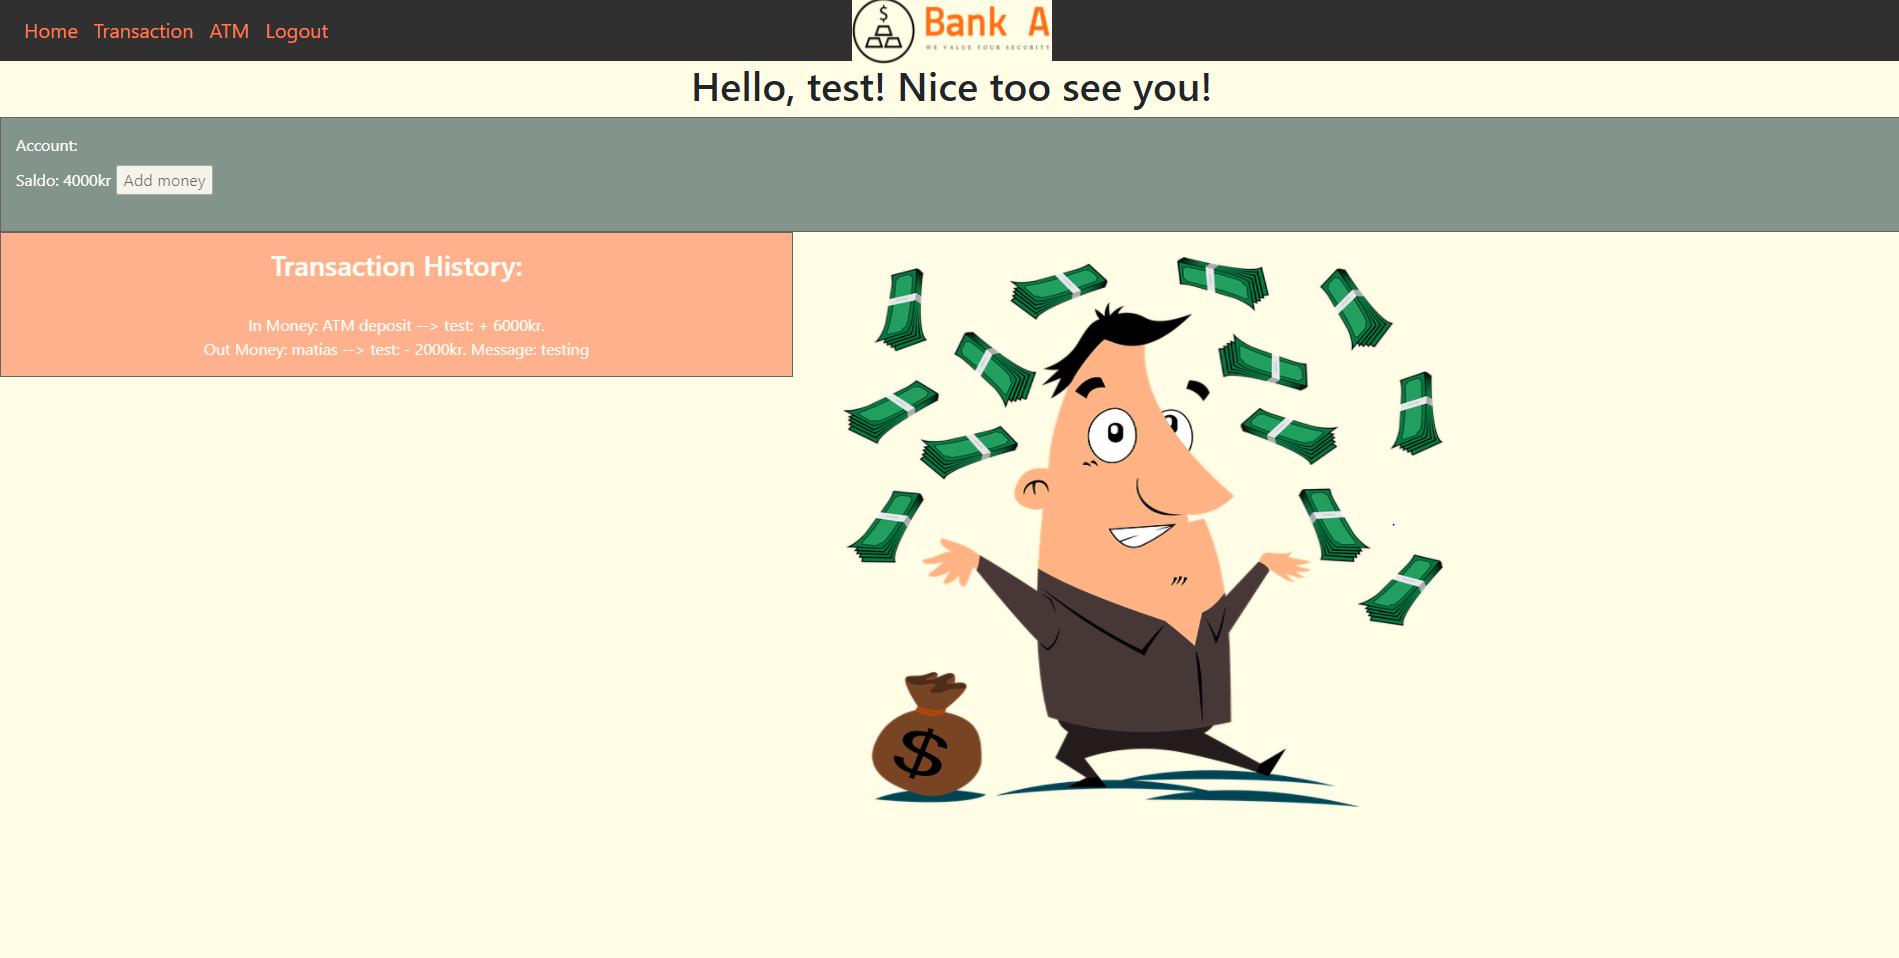
\includegraphics[width=\textwidth]{pics/pic3homeuser.PNG}
    \caption{User homepage}
\end{figure}

\begin{figure}[H]
    \centering
    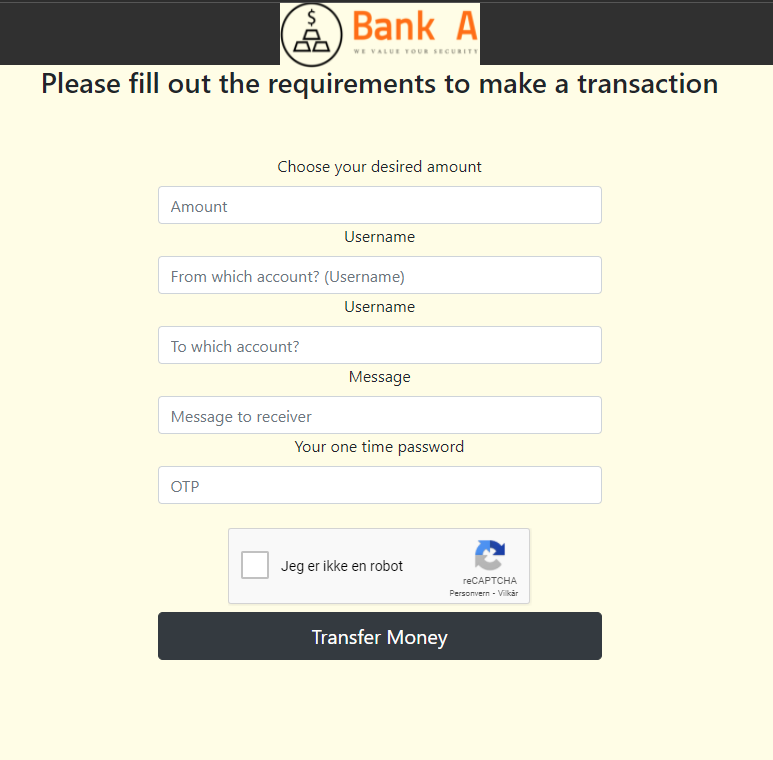
\includegraphics[width=\textwidth]{pics/pic 3.1.PNG}
    \caption{Transaction page}
\end{figure}

To transfer cash from your own bank account in the Transaction page, the user must know the username of the receiver, and in addition confirm his own. The user can also choose to send it with a message. This action must go through reCAPTCHA and 2FA authentication. 

ATM service simulates depositing cash in a local ATM to fill your account. This page looks like this, and must also confirm/verify the name of the user, reCAPTCHA and 2FA authentication. The limit is set to 10 000kr to have realistic values. The ATM page looks like this:

\begin{figure}[H]
    \centering
    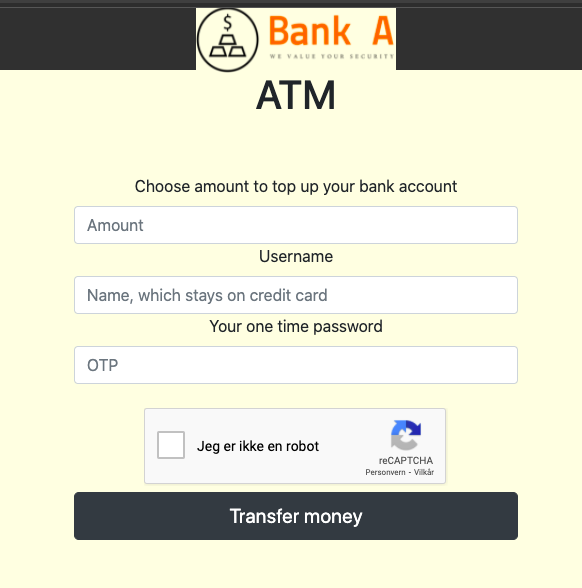
\includegraphics[width=\textwidth]{pics/atmPage.png}
    \caption{ATM page}
\end{figure}

\chapter{OWASP10 
}\label{kap:integrasjon}

%\begin{figure}[H]
%  \centering
%  \scalebox{0.6}{\includegraphics{prinsipp_num_int.pdf}}
%  \caption{Prinsippet for numerisk integrasjon av tidseriedata.
%    For hver ny måling $f(k)$ legges det inn et rektangel med bredde
%    $T_{s}(k-1)$, og totalarealet av rektanglene tilsvarer integralverdien. 
%    Figuren er hentet fra~\cite{Dre2020}.}
%  \label{fig:prinsipp_num_int}
%\end{figure}

\section{Problemstilling}

Problemstillingen i dette prosjektet har vært integrasjon i praktiske situasjoner. Ved numerisk integrasjon har vi tilgang bare til tidsseriesignalet, de vil si til data målt gjennom tid istedenfor å ha analytisk funksjon f(x) som kan integreres ved å finne antiderivert. 

Vi har lagt en simulasjon av «flow» i Matlab som skal være integrert. Simulert flow kan være både positiv og negativ, slik at vi kan måle økning eller reduksjon av den originale volumet. 
Simulasjon av flowsignalet har vi fått til ved å måle reflektert lys med lyssensoren og EV3 enheten fra Lego Mindstorm. Første måling er definert som ingen flow («nullflow»). Alle lysere verdier blir derfor positiv flow og mørkere verdier blir negativ flow.

\begin{figure}[H]
\centering
\scalebox{0.55}{}%\includegraphics{Kap4Fig1Bane.pdf}}
\caption{Ark brukt til simulasjon av flow}
\label{fig:kap1fig1bane}
\end{figure}

Vi har prøvd å oppnå målet ved å estimere arealet under flow ved å dele areal og summere det for å få anslag av arealet.

\section{Forslag til løsning}

Vi lagrer verdi og tid fra hver måling vi får fra lyssensoren i to forskjellige vektorer Lys og Tid. Disse to vektorer blir indeksert med helltallet «k» som starter fra 1 og øker med 1 for hver ny måling. Lysverdi fra første måling Tid(1) blir definert som «nullflow» og blir trukket fra alle lysverdier. Data etter subtraksjon blir lagret i Flow vektoren som også er indeksert med k.

\begin{figure}[H]
\centering
\scalebox{0.45}{}%\includegraphics{Kap1Fig2FlowLys.pdf}}
\end{figure}

Etterpå blir flowsignalet integrert ved hjelp av Euler forover og Trapes metodene. Begge to metodene handler om å dele areal under grafen inni blokker som ligger mellom tidspunkt av målingene på x-eksen. Areal av alle blokker summeres til slutt slik at vi får estimat av totalt areal fra x = 0 til x = k

\subsection{Kode for flow måling}

Flow blir implementert til matlab slikt:

\begin{python}
nullflow = Lys(1)
k = 1
while loop
   Flow(k) = Lys(k) - nullflow
   k = k + 1
end
\end{python}

Hvor Lys(k) er verdien vi får fra lyssensoren i måling nr k. På samme tid lagres tidspunkt av måling i egen vektor.

\subsection{Integrasjon ved Eulers forover metode}

\begin{figure}[H]
\centering
%\scalebox{0.5}{\includegraphics{eulerforovermetode.pdf}}
\end{figure}

I Euler forover metoden deles areal til rektangler som har tidsforskjell mellom to målingene som grunnflate og flowverdien som høyde.

\begin{lstlisting}
Volum(k) = Volum(k - 1) + Flow(k) * Tidsskritt
\end{lstlisting}

Hvor Tidsskritt er tid mellom måling k og måling (k - 1)

\begin{lstlisting}
Tidsskritt = Tid(k) - Tid(k - 1)
\end{lstlisting}

Formelen summerer forrige estimat av arealet med areal som kommer med ny flowmåling. Som du ser i figur 3 denne metoden tar ikke med trekanter som oppstår mellom grafen og rektangler, men estimatet blir mer nøyaktig med økt antall målinger i tidsintervallet.

\subsection{Integrasjon ved trapes metode}

\begin{figure}[H]
\centering
%\scalebox{0.5}{\includegraphics{integrasjonvedtrapes.pdf}}
\end{figure}

Trapes metoden tar gjennomsnittet mellom to flowverdier og omgjør areal mellom to tidspunkt til trapes. Denne trapesen har 2 lysverdier som 2 parallelle sider og Tidsskritt som høyde.
Areal av trapesen blir regnet ut med formel:

\begin{equation}
A = (a + b) * h/ 2   
\end{equation}

Etterpå blir areal av trapesen lagt til forrige estimat av arealet. 

\begin{lstlisting}
volum(k) = volum(k - 1) + (flow(k - 1) + flow(k)) * Tidsskritt / 2  
\end{lstlisting}

Siden denne formelen bruker gjennomsnittet mellom to flowverdiene, blir det mindre feil i estimat når stor variasjon mellom nåværende og forrige måling av flow skjer.

\section{Verifikasjon}

Her verifiserer vi estimat av volum med kalkulasjon gjort for hånd mellom punkt utlest i flowsignalet og volum.

\subsection{Verifikasjon del 1}

\begin{figure}[H]
\centering
%\scalebox{0.6}{\includegraphics{sammenligning.pdf}}
\end{figure}

Figur over viser at det er økning med 8 i tidsintervallet fra 9,028s til 11,57s

\begin{lstlisting}
Areal = Lys * Tid(slutt) - Lys * Tid(start)
Areal = Lys * Tidsskritt
\end{lstlisting}

\begin{verbatim}
Tidsskritt = 11,57 - 9,028 = 2,542
Lys = 8
Areal = 8 * 2,542 = 20,336
\end{verbatim}

Dette stemmer med avlesning fra volumet:
\begin{verbatim}
Stigning av volumet = 19,25 - (-1,042) = 20,292
\end{verbatim}

\subsection{Verifikasjon del 2, sinusfunksjonen}

Volum av sinusfunksjonen blir beregnet med formelen:

\begin{equation}
V(t) = \int a·sin(\omega·t)dt
\end{equation}

\begin{equation}
\omega = vinkelfrekvens  
\end{equation}

\begin{equation}
V(t) = -a · (1 /\omega) · cos(\omega·t) + C
\end{equation}

Hvor a står for amplituden og $\omega$ er vinkelfart. Konstanten C er volum ved Flow(1), altså 0.

\begin{figure}[H]
\centering
%\scalebox{0.3}{\includegraphics{sinuskurve.pdf}}
\end{figure}

Topp1 = 8,154s \\
Topp2 = 9,852s \\
Bunn = 8,981s

Amplitude = (Ymax - Ymin) / 2 \\
Amplitude = (6 - (-8)) / 2 \\
Amplitude = 7

Vinkelfart = 2pi / Tidsforskjellen mellom 2 topper \\
Vinkelfart = 2Pi / (9,852s - 8,154s) = 2Pi / 1,698 \\
Vinkelfart = 3,700 rad/s

Volumet ved 1. toppen (tid = 8,154s) vil være: \\
Volum(8,154) = - 7 * ( 1 / 3,700 ) * cos(3,700 * 8,154) \\
Volum(8,154) = -0,60350

Volumet ved 2. toppen (tid = 9,852s) vil være: \\
Volum(9,852) = - 7 * ( 1 / 3,700 ) * cos(3,700 * 9,852) \\
Volum(9,852) = -0,60245

Volum(8,154) og Volum(9,852) er praktisk likt, det betyr altså at beregningene av vinkelfart stemmer.

Toppunkt og bunnpunkt i denne funksjonen skjer når cosinus er lik 1 eller -1.
Bunnpunkt skjer ved cos(t)= 1, altså ved t = 0 \\
Volum(0) = - 7 * ( 1 / 3,700 ) * cos(3,700 * 0) \\
Volum(0) = -1,89

Areal ved minimalpunkt I denne sinusfunksjonen er -1.88, men den er bare halvparten av «negativ» flow, som stopper mellom bunnpunkt og topppunkt. Derfor må vi gange areal som vi får i bunnpunkt med 2.

\begin{figure}[H]
\centering
%\scalebox{0.45}{\includegraphics{Kap1Fig7.pdf}}
\end{figure}

-1,89 * 2 = -3,78

Dette stemmer med data fra volumgrafen i figur 6: \\
35,83 - 32,1 = 3,73

Volumet har blitt mindre med 3,73, som er veldig nærme forventet 3,78.


\section{Integrasjonsmetoder i eksterne funksjoner}

Til slutt har vi lagret funksjoner i separate .mat filer slik at koden for integrering kan brukes i andre prosjekter.

Her er kallet til funksjoner EulerForward:
\begin{lstlisting}
volumEuler(k) = EulerForward(volum(k-1), flow(k-1), Ts(k-1))
\end{lstlisting}

EulerForward trenger forrige areal estimat, forrige flowverdien og tidsskritt mellom aktuell og forrige måling.

Kallet til Trapesfunksjonen ses ut slik: 
\begin{lstlisting}
volumTrapes(k) = Trapes(volum(k-1),flow(k-1:k),Ts(k-1))
\end{lstlisting}

Trapes funksjonen trenger å vite nåværende flowverdien i tillegg til forrige areal estimat, forrige flowverdien og tidsskritt mellom aktuell og forrige måling.


\begin{figure}[H]
\centering
%\scalebox{0.3}{\includegraphics{sammenligningavtofunk.pdf}}
\end{figure}
%\input{konklusjon.tex}


% Første linje er bibliografistilen, her finner flere varianter som du
% prøve. Andre linje er selve filen med dine referanser. Siste linje
% legger bibliografi inn i innholdsfortegnelsen. 

\bibliographystyle{plain}
%\bibliography{referanser.bib}
\addcontentsline{toc}{chapter}{Bibliografi} 

\appendix

\end{document}


